\section{Auswertung}
\label{sec:Auswertung}
In der folgenden \autoref{tab:1} werden die Materialeigenschaften der Grundplatte aufgelistet.
\begin{table}[H]
  \centering
  \caption{Materialeigenschaften der Grundplatte. \cite{V204}}
  \label{tab:1}
  \sisetup{table-format=1.2}
  \begin{tabular}{l S S S S S }
    \toprule
    {$\text{Material}$} & {$l [\si{\centi\meter}]$} & {$b [ \si{\centi\metre}]$} & {$h[\si{\centi\metre}]$} & {$\rho [\si{\kilo\gram\per\metre\tothe{3}}$]} & {$c [\si{\joule\per\kilo\gram\per\kelvin}]$} \\
    \midrule
    Messing  & 9 & 1.2 & 0.4 & 8520 & 385 \\
    Messing  & 9 & 0.7 & 0.4 & 8520 & 385 \\
    Aluminium  & 9 & 1.2 & 0.4 & 2800 & 830 \\
    Edelstahl  & 9 & 1.2 & 0.4 & 8000 & 400 \\
    \bottomrule
  \end{tabular}
\end{table}


\subsection{Statische Messung}
\label{subsec:aus_stat}
Wie in \autoref{subsec:durch_stat} beschrieben, wird eine statische Messung der Temperaturverläufe an den Stäben durchgeführt. 
Die Daten werden in folgenden Diagrammen dargestellt und ausgewertet.

\begin{figure}[H]
  \begin{subfigure}{\textwidth}
  \centering
  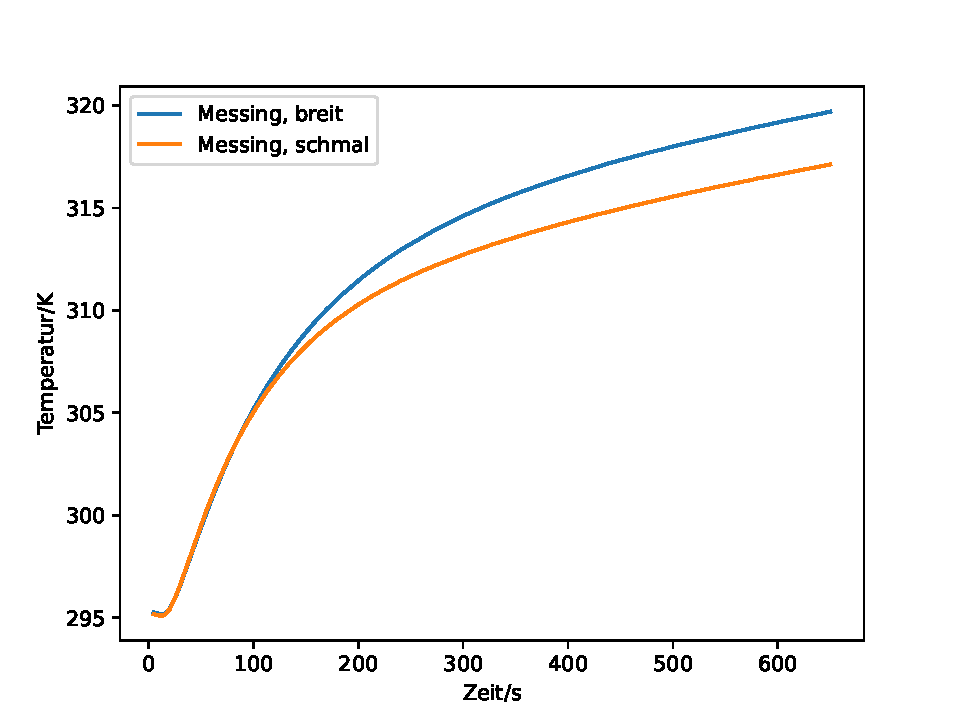
\includegraphics[height=6cm]{content/verlauf_mess.pdf}
  \caption{Temperaturverlauf der Messingstäbe.(fern)}
  \label{fig:mess}
  \end{subfigure}
  \hfill
  \begin{subfigure}{\textwidth}
  \centering
  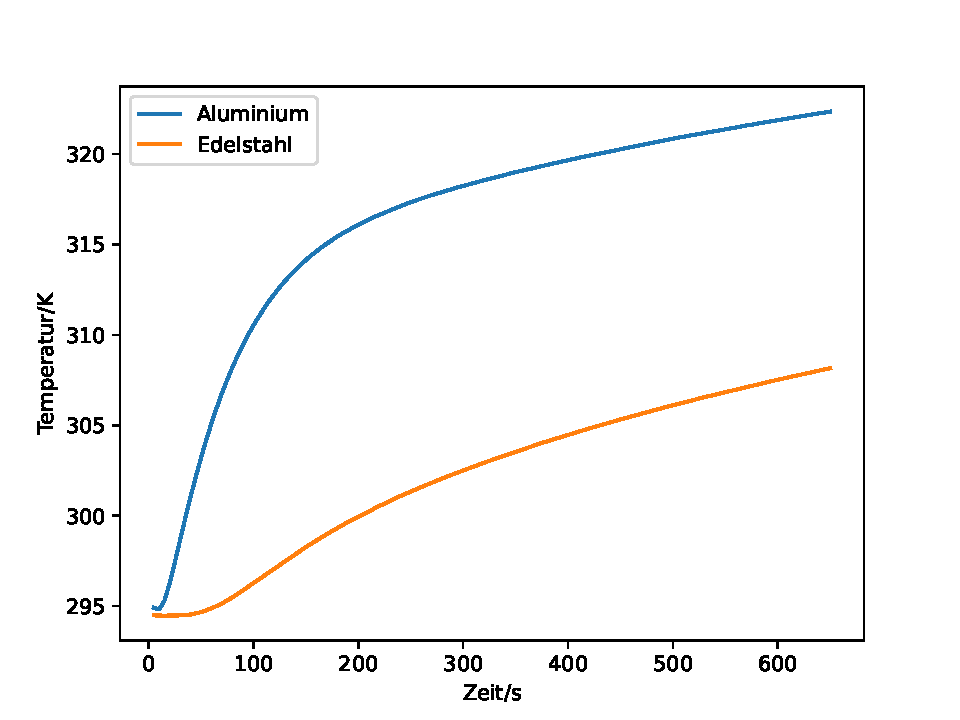
\includegraphics[height=6cm]{content/verlauf_alu_edel.pdf}
  \caption{Temperaturverlauf des Aluminium- und Edelstahlstabs.(fern)}
  \label{fig:alu_edel}
  \end{subfigure}
  \caption{Temperaturverläufe der Stäbe an den fernen Thermoelementen.}
  \label{fig:fern}
\end{figure}
\noindent Zunächst wurden die Temperaturen an den fernen Thermoelementen über einen Zeitraum von $\qty{650}{\second}$ aufgenommen.
Die Temperaturverläufe aller $4$ untersuchten Stäbe weisen Gemeinsamkeiten auf. So zeigt der Graph in \autoref{fig:fern},
dass bei allen Metallen die Temperatur initial stark steigt und sich mit zunehmender Zeit einem Sättigungswert annähert.
Der Temperaturanstieg ist bei Edelstahl allerdings deutlich langsamer als bei den übrigen Metallen und auch der Sättigungswert ist hier deutlich niedriger.
Bei den beiden Messingstäben sind sehr ähnliche Temperaturverläufe zu beobachten, wobei die Kurve des breiten Stabs zu einem späteren Zeitpunkt abflacht als die des schmalen Stabs.


\begin{table}[H]
  \centering
  \caption{Temperaturen der Stäbe nach 650s.}
  \label{tab:650s}
  \begin{tabular}{l S[table-format=3.2]}
    \toprule
    {Material} & {Temperatur [K]}\\
    \midrule
    {Messing, breit} & 319.70\\
    {Messing, schmal} & 317.12\\
    {Aluminium} & 322.35\\
    {Edelstahl} & 308.15\\
    \bottomrule
  \end{tabular}
\end{table}
\noindent Zur Bewertung der Wärmeleitung der Stäbe wurde die Temperatur am Ende der statischen Messung erhoben und in einer Tabelle dargestellt.
Aus den Werten in \autoref{tab:650s} lässt sich erkennen, dass Aluminium von den untersuchten Metallen die beste Wärmeleitfähigkeit besitzt
und Edelstahl die Wärme am schlechtesten leitet.

\begin{table}[H]
  \centering
  \caption{Wärmeströme zu verschiedenen Messzeiten.}
  \label{tab:dQ/dt}
  \sisetup{table-format=3.3}
  \begin{tabular}{S[table-format=3.0] S S S S S S S}
    \toprule
    & \multicolumn {3}{c}{Messing,breit}& \multicolumn {3}{c}{Messing,schmal}\\
    \cmidrule(lr){2-4}\cmidrule(lr){5-7}
    \multicolumn{1}{c}{Messzeitpunkt $t$ / $\si{s}$}& \multicolumn{1}{c}{$T_1\mathbin{/}K$} & \multicolumn{1}{c}{$T_2\mathbin{/}K$} & \multicolumn{1}{c}{$\frac{\Delta Q}{\Delta t}\mathbin{/}\si{W}$}  &\multicolumn{1}{c}{$T_3\mathbin{/}K$} & \multicolumn{1}{c}{$T_4\mathbin{/}K$} & \multicolumn{1}{c}{$\frac{\Delta Q}{\Delta t}\mathbin{/}\si{W}$}\\ 
    \midrule
    50 &299.40&306.23&-1.235&307.85&299.52&-0.879\\
    200 &311.45&315.15&-0.669&315.21&310.28&-0.520\\
    350 &315.68&318.31&-0.476&317.60&313.57&-0.425\\
    500 &317.99&320.35&-0.427&319.38&315.55&-0.404\\
    650 &319.70&321.96&-0.409&320.89&317.12&-0.398\\
    \toprule
    & \multicolumn {3}{c}{Aluminium}& \multicolumn {3}{c}{Edelstahl}\\
    \cmidrule(lr){2-4}\cmidrule(lr){5-7}
    \multicolumn{1}{c}{Messzeitpunkt $t$ / $\si{s}$}&{$T_5\mathbin{/}K$} & \multicolumn{1}{c}{$T_6\mathbin{/}K$} & \multicolumn{1}{c}{$\frac{\Delta Q}{\Delta t}\mathbin{/}\si{W}$}  &\multicolumn{1}{c}{$T_7\mathbin{/}K$} & \multicolumn{1}{c}{$T_8\mathbin{/}K$} & \multicolumn{1}{c}{$\frac{\Delta Q}{\Delta t}\mathbin{/}\si{W}$} \\
    \midrule
    50 &303.19&308.64&-2.067&303.04&294.66&-0.268\\
    200 &316.09&318.32&-0.846&312.29&299.94&-0.395\\
    350 &319.00&320.70&-0.645&314.59&303.54&-0.354\\
    500 &320.85&322.43&-0.599&316.49&306.11&-0.332\\
    650 &322.35&323.91&-0.592&318.16&308.15&-0.320\\
    \bottomrule
  \end{tabular}
\end{table}
\noindent In der \autoref{tab:dQ/dt} sind die mithilfe von \autoref{eqn:Wärmemenge} berechneten Wärmeströme der
verschiedenen Metalle zu fünf unterschiedlichen frei gewählten Messzeitpunkten zu sehen.

\begin{figure}[H]
  \begin{subfigure}{\textwidth}
  \centering
  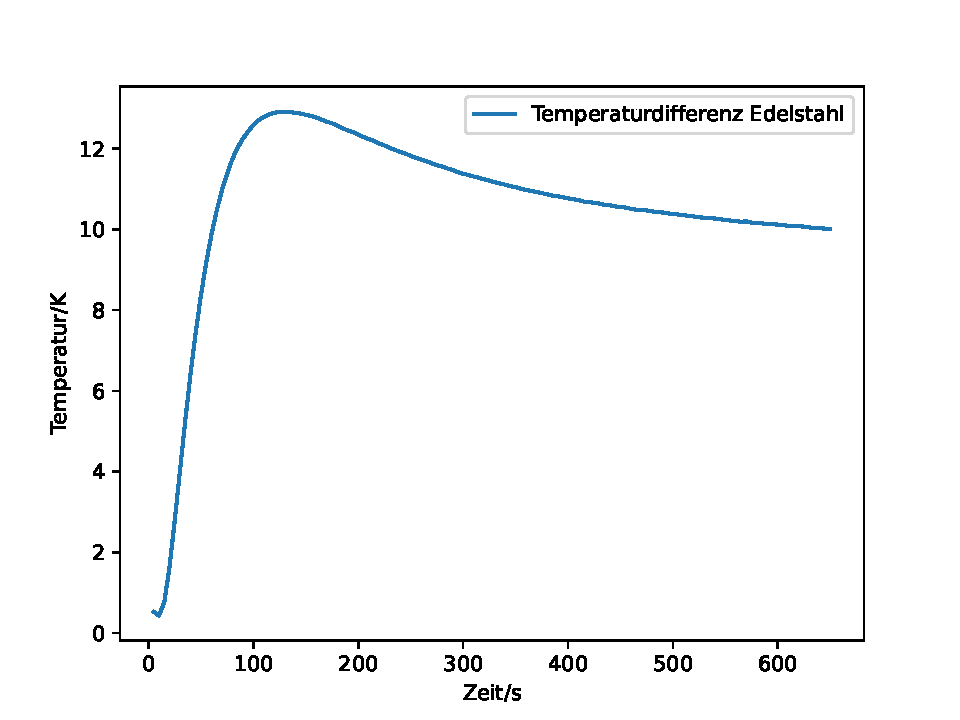
\includegraphics[height=7cm]{content/differenz_edel.pdf}
  \caption{Verlauf der Temperaturdifferenz am Edelstahlstab.}
  \label{fig:diff_edel}
\end{subfigure}
\begin{subfigure}{\textwidth}
  \centering
  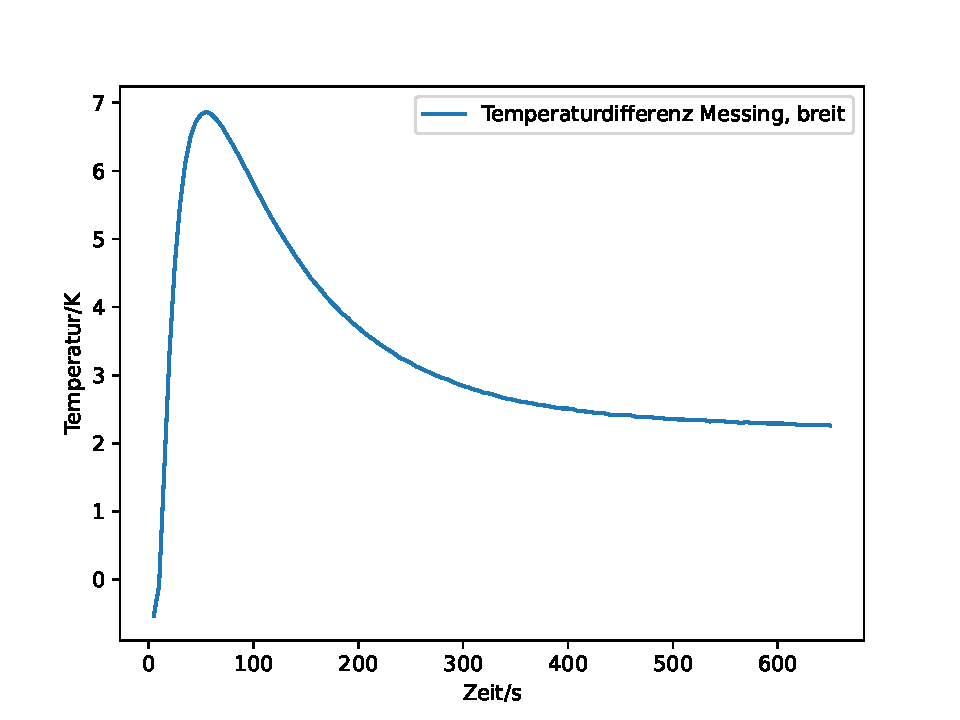
\includegraphics[height=7cm]{content/differenz_mess.pdf}
  \caption{Verlauf der Temperaturdifferenz am breiten Messingstab.}
  \label{fig:diff_mess}
\end{subfigure}
\caption{Verlauf der Temperaturdifferenzen zwischen den Thermoelementen.}
\label{fig:diff}
\end{figure}

\noindent In \autoref{fig:diff} sind die Verläufe der Temperaturdifferenzen zwischen den Thermoelementen auf dem breiten Messingstab, sowie dem Edelstahlstab dargestellt.
Es lässt sich erkennen, dass die Kurve der Differenz bei beiden Stäben zunächst stark bis zu einem Hochpunkt ansteigt. Danach fällt sie bis sie sich einem Sättigungswert annähert.
Beim Messingstab ist die Differenz allerdings ab dem Hochpunkt der Kurve deutlich niedriger als beim Edelstahlstab.
Die Temperaturdifferenz am Hochpunkt der Kurve bei Edelstahl erreicht einen Wert von über 12 K, wobei der Wert am Hochpunkt der Messingkurve unter 7 K liegt.

\subsection{Dynamische Messung}
\label{subsec:aus_dyn}
Wie in \autoref{subsec:durch_dyn} beschrieben, werden mehrere dynamische Messungen der Temperaturverläufe an den Stäben durchgeführt. 


\subsubsection{Messung mit Periodendauer 80s}
\label{subsec:aus_dyn80}

Zunächst wurde die Messung nach dem Angström-Verfahren mit einer Periodendauer von $\qty{80}{\second}$ durchgeführt.
Die Werte an den Thermoelementen am breiten Messingstab und am Aluminiumstab werden in \autoref{fig:mess_dyn} und \autoref{fig:alu_dyn} dargestellt.


\begin{figure}[H]
  \centering
  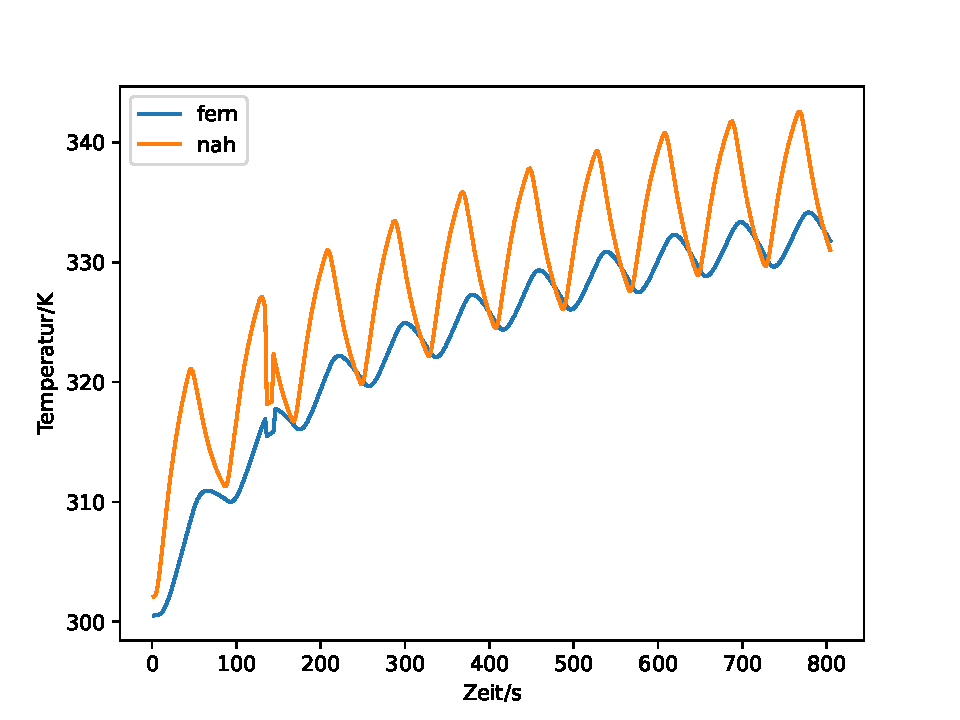
\includegraphics[height=9.5cm]{content/dyn_80_mess.pdf}
  \caption{Temperaturverlauf des breiten Messingstabs.}
  \label{fig:mess_dyn}
\end{figure}
\begin{figure}[H]
  \centering
  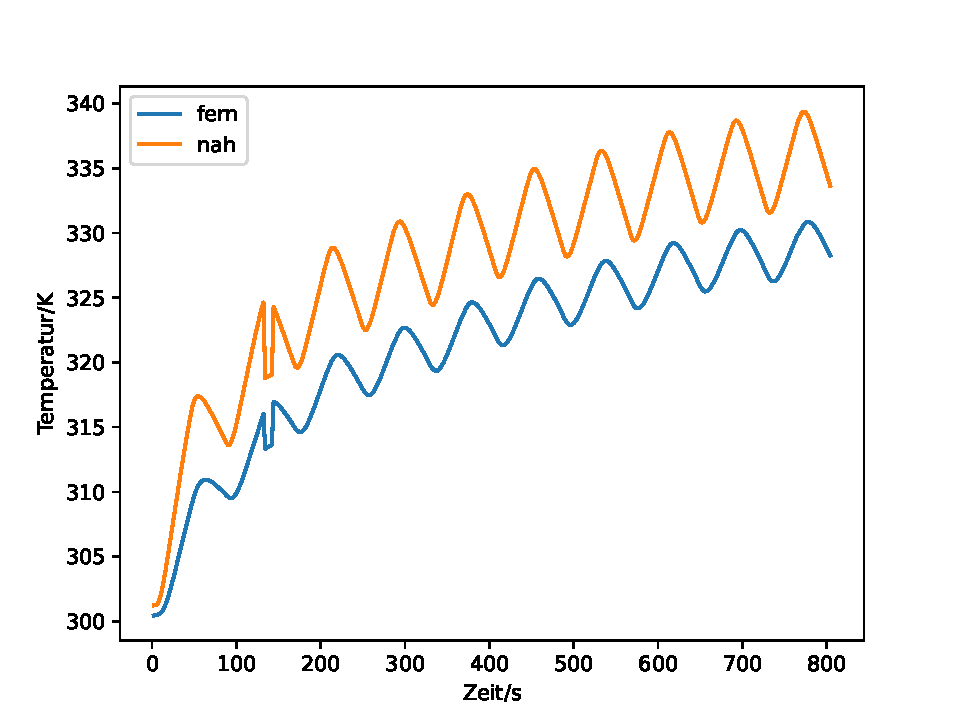
\includegraphics[height=9.5cm]{content/dyn_80_alu.pdf}
  \caption{Temperaturverlauf des Aluminiumstabs.}
  \label{fig:alu_dyn}
\end{figure}

\noindent Anhand der Graphen wurden die Amplituden, sowie die Phasendifferenzen aus den Abständen der Wellenhochpunkte beider Wellen bestimmt.
 Die Rechnungen wurde mithilfe der Phythonmodule Matplotlib \cite{matplotlib}, Numpy \cite{numpy}, Scipy \cite{scipy} und Uncertainties\cite{uncertainties} durchgeführt, weswegen die Fehler verschwindend gering sind und vernachlässigbar sind.
	
\begin{table}[H]
	\centering
	\caption{Amplituden und Phasendifferenzen Messing und Aluminium.}
	\label{tab:AuP}
  \sisetup{table-format=2.3}
	\begin{tabular}{l S S S[table-format=2.0] S S S[table-format=2.0]}
		\toprule
    & \multicolumn{3}{c} {Messing} & \multicolumn{3}{c} {Aluminium}\\
    \cmidrule(lr){2-4}\cmidrule(lr){5-7}
		&{$A_{nah}\mathbin{/}K$} & {$A_{fern}\mathbin{/}K$} &{$\Delta t \mathbin{/}\si{\second}$}&{$A_{nah}\mathbin{/}K$} & {$A_{fern}\mathbin{/}K$} &{$\Delta t \mathbin{/}\si{\second}$}\\
		\cmidrule(lr) {2-4}\cmidrule(lr) {5-7}
		&9.5&5.21&20   & 11.51 & 8.075 & 10 \\
    &7.91&3.865&16 & 9.43 & 5.505 & 4 \\
    &7.16&3.07&14  &8.46 & 4.64 & 6 \\
    &6.83&2.635&12 & 8.19 & 4.18 & 8 \\
    &6.865&2.61&12 & 8.12 & 4.28 & 8 \\
    &6.67&2.48&10  & 8.05 & 4.19 & 8 \\
    &6.595&2.41&10 & 7.965 & 4.095 & 6 \\
    &6.615&2.395&10& 7.98 & 4.19 & 8 \\
    &6.405&2.225&10& 7.805 & 3.95 & 6 \\
    &6.45&2.265&10 & 7.817 & 3.915 & 6 \\
    \cmidrule(lr) {2-4}\cmidrule(lr) {5-7}
    {Mittelwert}&7.100 &2.920 &12.400 & 8.533 & 4.702 & 7.000\\
		\bottomrule
	\end{tabular}
\end{table}	

\pagebreak 
\noindent Aus den Werten in \autoref{tab:AuP} kann mithilfe von \autoref{eqn:kappa} die Wärmeleitfähigkeit berechnet werden.
Der Fehler wird nach der Gauß'schen Fehlerfortpflanzung mit 
\begin{equation}
  \label{eqn:Gauß}
  \Delta \kappa = \sqrt{\biggl(\frac{\partial \kappa}{\partial \Delta t}\biggr)^2\cdot (\Delta (\Delta t))^2+
  \biggl(\frac{\partial \kappa}{\partial A_\text{nah}}\biggr)^2\cdot (\Delta  A_\text{nah} )^2+
  \biggl(\frac{\partial \kappa}{\partial A_\text{fern}}\biggr)^2\cdot (\Delta  A_\text{fern})^2} 
 \end{equation}
 bestimmt.

\noindent Die Wärmeleitfähigkeit beträgt somit:
\begin{align*}
  \kappa_{\text{Messing}}&=\qty{133.95 +- 63.92}{\watt\per\meter\per\kelvin}\\
  \kappa_{\text{Aluminium}}&=\qty{250.72 +- 140.93}{\watt\per\meter\per\kelvin}
\end{align*}

\subsubsection{Messung mit Periodendauer 200s}
\label{subsubsec:aus_dyn200}

Analog zu \autoref{subsec:aus_dyn80} wurde die Messung nach dem Angström-Verfahren mit einer Periodendauer von $\qty{200}{\second}$ durchgeführt.
Die Werte an den Thermoelementen am Edelstahlstab werden in \autoref{fig:edel_dyn} dargestellt.

\begin{figure}[H]
  \centering
  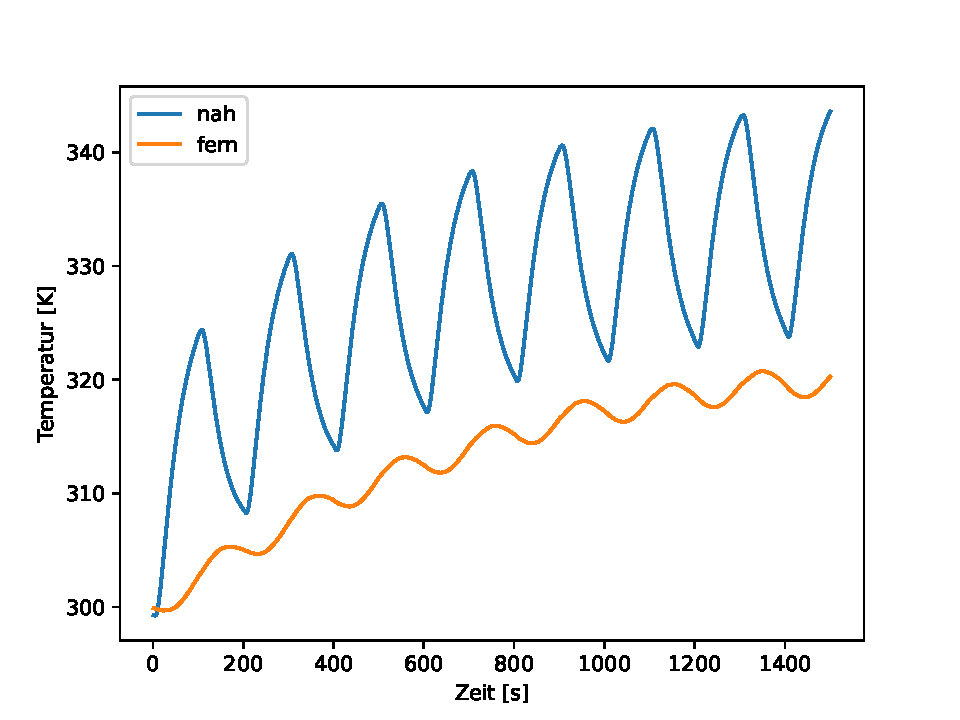
\includegraphics[height=9.5cm]{content/dyn_2.pdf}
  \caption{Temperaturverlauf des Edelstahlstabs.}
  \label{fig:edel_dyn}
\end{figure}

Auch hier werden die Amplituden und Phasendifferenzen berechnet.
\begin{table}[H]
	\centering
	\caption{Amplituden und Phasendifferenzen Edelstahl.}
	\label{tab:AuPE}
  \sisetup{table-format=2.3}
	\begin{tabular}{l S S S[table-format=2.0]}
		\toprule
		&{$A_{nah}$ [K]} & {$A_{fern}$ [K]} &{$\Delta t [\si{\second}]$}\\
		\cmidrule(lr) {2-4}
		& 12.57 & 2.81& 64 \\
    & 11.39& 2.56 & 64\\
    &10.85& 2.17 & 54\\
    & 10.585 & 2.065 & 50 \\
    & 10.365& 1.885& 50\\
    & 10.205& 1.665& 46\\
    & 10.158& 1.595 & 40\\
    \cmidrule(lr) {2-4}
    {Mittelwert}&10.879&2.107 &52.571 \\
		\bottomrule
	\end{tabular}
\end{table}	

Die Wärmeleitfähigkeit von Edelstahl wird nun berechnet zu:
\begin{align*}
  \kappa_{\text{Edelstahl}}&=\qty{10.97 +- 1.52}{\watt\per\meter\per\kelvin}\\
  \end{align*}

Nach \autoref{eqn:welle} lassen sich die Wellenlängen der Temperaturwellen bestimmen.
\begin{table}
  \centering
  \caption{Wellenlängen der Temperaturwellen.}
  \label{tab:Wellenlänge}
  \sisetup{table-format=1.3}
  \begin{tabular}{l
      S@{${}\pm{}$}
      S
      }
      \toprule
      \multicolumn{1}{l}{Material}&\multicolumn{2}{p{3cm}}{Wellenlänge$\, [\si{\m}]$} \\
      \midrule
      Messing & 0.203 & 0.048\\
      Aluminium & 0.329 & 0.093\\ 
      Edelstahl & 0.093 & 0.006\\
      \bottomrule
  \end{tabular}
\end{table}

Die Frequenzen $f=1/T$ betragen $f_{80s}=\qty{0.0125}{\second\tothe{-1}}$ und $f_{200s}=\qty{0.005}{\second\tothe{-1}}$.

\pagebreak



